\documentclass[sigconf]{acmart}

\usepackage{booktabs} % For formal tables
\usepackage{amsmath,amssymb}
% \usepackage{cite}   % importing cite is throwing errors for some reason
\usepackage{color}
\usepackage{enumerate}
\usepackage{multicol}

\usepackage{tikz}
\tikzset{
  treenode/.style = {shape=rectangle, rounded corners,
                     draw, align=center,
                     top color=white, bottom color=blue!20},
  root/.style     = {treenode, font=\Large, bottom color=red!30},
  env/.style      = {treenode, font=\ttfamily\normalsize},
  dummy/.style    = {circle,draw}
}

\usepackage{tikz-qtree}
\usepackage{tikz-qtree-compat}
\usetikzlibrary{positioning}
\usepackage{ textcomp }
% Get todos to render properly
\usepackage[obeyFinal]{easy-todo}

% Add package for ::= symbol, can't compile to pdf for some reason
% \usepackage{txfonts}

% Add package for well rendered quotations
\usepackage{dirtytalk}
\usepackage{hyperref}
\usepackage{graphicx}

\usepackage{lambda}

% correct bad hyphenation here
\hyphenation{op-tical net-works semi-conduc-tor}

% Copyright
%\setcopyright{none}
%\setcopyright{acmcopyright}
%\setcopyright{acmlicensed}
\setcopyright{rightsretained}
%\setcopyright{usgov}
%\setcopyright{usgovmixed}
%\setcopyright{cagov}
%\setcopyright{cagovmixed}


% DOI
\acmDOI{10.475/123_4}

% ISBN
\acmISBN{123-4567-24-567/08/06}

%Conference
\acmConference[Seattle'2017]{SIGCSE}{March 2017}{Seattle, Washington USA} 
\acmYear{2017}
\copyrightyear{2017}

\acmPrice{15.00}


\begin{document}
\title{A Domain Analysis of Data Structure and Algorithm Explanations in the Wild}


\author{Jeffrey Young} 
\affiliation{%
 \institution{Oregon State University}
 \department{School of EECS}
 \city{Corvallis} 
 \state{Oregon}
 \country{USA}}
\author{Eric Walkingshaw} 
\affiliation{%
 \institution{Oregon State University}
 \department{School of EECS}
 \city{Corvallis} 
 \state{Oregon}
 \country{USA}}
\todo{anonymize authors}


\begin{abstract}
  Explanations of data structures and algorithms are complex interactions of
  several notations, including natural language, mathematics, pseudocode, and
  diagrams. Currently, such explanations are created ad hoc using a variety of
  tools, and the resulting artifacts are static, reducing explanatory value. We
  envision a domain-specific language for developing rich, interactive
  explanations of data structures and algorithms. In this paper, we analyze this
  domain to sketch requirements for our language. We perform a grounded theory
  analysis, to generate a qualitative coding system for explanation artifacts
  collected online. We show that grounded theory provides a robust methodology
  for analyzing qualitative objects and that the resultant coding system forms
  the skeleton of a domain-specific language. This work is part of our effort to
  develop the paradigm of explanation-oriented programming, which shifts the
  focus of programming from computing results to producing rich explanations of
  how those results were computed.
  \todo{I want to say something here about using formal qualitative methods to
    expand the reach of computer science}
  \todo{do we mention explanation trees in the abstract and pre-order traversals?}
\end{abstract}

%
% The code below should be generated by the tool at
% http://dl.acm.org/ccs.cfm
% Please copy and paste the code instead of the example below. 
%
\todo{CCSXML}
\begin{CCSXML}
<ccs2012>
 <concept>
  <concept_id>10010520.10010553.10010562</concept_id>
  <concept_desc>Computer systems organization~Embedded systems</concept_desc>
  <concept_significance>500</concept_significance>
 </concept>
 <concept>
  <concept_id>10010520.10010575.10010755</concept_id>
  <concept_desc>Computer systems organization~Redundancy</concept_desc>
  <concept_significance>300</concept_significance>
 </concept>
 <concept>
  <concept_id>10010520.10010553.10010554</concept_id>
  <concept_desc>Computer systems organization~Robotics</concept_desc>
  <concept_significance>100</concept_significance>
 </concept>
 <concept>
  <concept_id>10003033.10003083.10003095</concept_id>
  <concept_desc>Networks~Network reliability</concept_desc>
  <concept_significance>100</concept_significance>
 </concept>
</ccs2012>  
\end{CCSXML}

\ccsdesc[500]{Computer systems organization~Embedded systems}
\ccsdesc[300]{Computer systems organization~Redundancy}
\ccsdesc{Computer systems organization~Robotics}
\ccsdesc[100]{Networks~Network reliability}


\keywords{ACM proceedings, \LaTeX, text tagging}
\todo{figure out keywords}

\maketitle

\section{Introduction}
\label{sec:intro}

Data structures and algorithms are at the heart of computer science and must be
explained to each new generation of students. A pressing question is: How can we
do this effectively?

In this paper, we focus on the \emph{artifacts} that constitute or support
explanations of data structures and algorithms (hereafter just ``algorithms''),
which can be shared and reused.
%
For verbal explanations, such as a lecture, the supporting artifact might be
the associated slides. For written explanations, the artifact is the
explanation as a whole, including the text and any supporting figures.
%
Explanation artifacts associated with algorithms are interesting because they
typically present a complex interaction among many different notations,
including natural language, mathematics, pseudocode, executable code, various
kinds of diagrams, animations, and more.


Currently, explanation artifacts for algorithms are created ad hoc using a
variety of tools and techniques, and the resulting explanations tend to be
static, reducing their explanatory value.
%
Although there has been a substantial amount of work on algorithm visualization~
\cite{Gloor92,Gloor97,HDS02, shaffer2010algorithm, HANSEN2002291, KANN1997223},
and tools exist for creating these kinds of supporting artifacts, there is no
good solution for creating integrated, multi-notational explanations as a whole.
Similarly, although some algorithm visualization tools provide a means for the
student to tweak the parameters or inputs to an algorithm to generate new
visualizations, they do not support creating cohesive interactive explanations
that correspondingly modify the surrounding explanation or that allow the
student to respond to or query the explanation in other ways.
%
To fill this gap, we envision a \emph{domain-specific language} (DSL) that
supports the creation of rich, interactive, multi-notational artifacts for
explaining algorithms.
%
The development of this DSL is part of a larger effort to explore the new
paradigm of \emph{explanation-oriented programming}, briefly described in
Section~ \ref{sec:back:xop}.


The intended users of the envisioned DSL are CS educators who want to create
\emph{interactive artifacts} to support the explanation of algorithms. These
users are experts on the corresponding algorithms, and also trained and skilled
programmers. The produced explanation artifacts might supplement a lecture or
be posted to a web page as a self-contained (textual and graphical)
explanation.
%
The DSL should support pedagogical methods directly through built-in
abstractions and language constructs. It should also support a variety of forms
of student interaction. For example, teachers should be able to define
equivalence relations enabling users to automatically generate variant
explanations~\cite{EW13jvlc}, to build in specific responses to anticipated
questions, and to provide explanations at multiple levels of abstraction.


This paper represents a formative step toward this vision. We conduct a
\emph{qualitative analysis} of our domain in order to determine the form and
content of the explanation artifacts that educators are already creating.
%
We base our analysis on an established qualitative research method called
\emph{grounded theory} in order to better understand how well existing artifacts
explain complex topics


More specifically, we collect 15 explanation artifacts from the internet,
consisting of only lecture notes that explain two algorithms and one
data structure commonly covered in undergraduate computer science courses:
Dijkstra's shortest path algorithm~\cite[pp.~137--142]{KT06}, merge sort
\cite[210--214]{KT06}, and AVL trees \cite[pp.~458--475]{KnuthArt3}.
%
We analyze these artifacts through the application of grounded
theory\cite{Strauss67discoveryof}, a formal method for analyzing qualitative
data that originated in sociological research. Through the application of
grounded theory, we develop a coding system that captures the structure of
explanation for each document. An overview of the coding system is given in
Section \ref{sec:res:sys}.

% We analyze these artifacts by applying a classic pedagogical theory by Bellack
% et al.~\cite{bellack1966language} that describes the patterns of language used
% in the process of teaching. Bellack et al.\ define a typology for coding
% transcripts of teacher and student verbalizations during teaching. An overview
% of the typology is given in Section~\ref{sec:back:typ}.


This paper makes the following contributions:
%
\begin{enumerate}[C1.]

\item \label{contrib:method}
  We provide a case study on analyzing \emph{qualitative data} through the
  application of a formal research method \emph{grounded theory}, that is not
  part of the computer science parlance.

\item \label{contrib:data}
%
We provide a coded qualitative data set of explanation artifacts, using the
system defined in C\ref{contrib:codes} applied to our sample of 15 collected
explanation artifacts (Section~\ref{sec:exp:data}).

\item \label{contrib:codes}
%
\todo{decide if we need to split this contribution up}
We provide a coding system for analyzing \emph{explanation artifacts} in the
form of lecture notes, and we show that through the application of the coding
system, each such artifact forms a tree structure, which we have termed a
\emph{explanation tree} (Section \ref{sec:res:xopTree}).


\item \label{contrib:dsl}
%
  We describe how a coding system grounded in data can directly provide a
  semantics basis for a DSL and argue for the advantages of such an approach
  (Section~\ref{sec:res:dsl}).
%
\end{enumerate}

\noindent

\section{Background}
\label{sec:back}

In this section, we put the present work into context by the describing the
paradigm of \emph{explanation-oriented programming} in
Section~\ref{sec:back:xop}, the exploration of which is an underlying
motivation of our work, and by introducing the methodology of grounded theory
~\cite{Strauss67discoveryof} in Section~\ref{sec:back:gt}, which is the
theoretical foundation of our coding system.

\subsection{Explanation-oriented programming}
\label{sec:back:xop}

\emph{Explanation-oriented programming} (XOP) is a new programming paradigm
% originally proposed at VL/HCC~2008~\cite{EW08vl},
where the primary output of a program is not a set of computed values, but an
\emph{explanation of how} those values were
computed~\cite{EW08vl,EW09dsl,EW09vl,WE11dsl,EW13jvlc}.
%
A high-level goal of this work is to further develop the paradigm of XOP
through the development of a specific DSL.


Programming languages for XOP should not merely produce explanations as a
byproduct, but should provide abstractions and features specific to the
creation of interactive explanation artifacts. For example, they should provide
facilities for creating application-specific notations and visualizations
(which are widespread in explanations of algorithms), and for describing
alternative explanations produced in response to user input, for example, at
different levels of abstraction, by parameterization, or generated by
explanation equivalence laws~\cite{EW13jvlc}. Additionally, languages for XOP
should help guide the programmer toward the creation of \emph{good}
explanations.


The need for interactive explanation artifacts is motivated by the observation
that there is a trade-off between personal explanations and traditional
explanation artifacts, which can be partially bridged by XOP programs viewed as
rich, interactive explanation artifacts.
%
A good \emph{personal explanation} is useful because the explainer can
\emph{respond} to the student, adjusting the pace and strategy as necessary.
For example, the teacher can answer questions, rephrase parts of an
explanation, and provide additional examples as needed.
%
Unfortunately, good personal explanations are a scarce resource. First, there
are limited number of people who can provide high quality personal explanations
on a topic. Second, a personal explanation is usually ephemeral and so cannot
be directly shared or reused.
%
Since personal explanations are hard to come by, many students learn from
\emph{impersonal explanation artifacts}, such as recorded lectures, textbooks
and online written nd graphical resources.
%
These impersonal explanations lack the interaction and adaptability of personal
explanations, but have the advantage of being easy to massively share and reuse
via libraries and the internet.


In-person lectures, such as those covering algorithms in most undergraduate
computer science programs, exist at a midway point between impersonal and
personal explanations, perhaps closer to the personal end of the spectrum.
These \emph{classroom explanations} are adaptable---students can ask questions
in class, the teacher can respond, and explanations can be adapted on the fly
if students are confused---but they are not as adaptable as personal
explanations since the teacher must accommodate many students at once.
Classroom explanations are more efficient than personal explanations since they
are shared amongst many students, but not as efficient as impersonal
explanations since they are still ephemeral and therefore difficult to reuse.


We target another midway point, a bit closer to the impersonal end of the
spectrum, of \emph{interactive explanation artifacts} that provide as much of
the responsiveness and adaptability of personal explanations as possible, but
which can still be massively shared and reused online. Such an explanation
artifact would be quite expensive to produce with current tools since an
\emph{explanation designer} must not only construct a high quality initial
explanation and corresponding visualizations, but also anticipate and
explicitly program in responses to queries by the student.
%
We expect that DSLs for XOP can help alleviate this burden.


% To help realize this vision, our medium-term goal is to design a
% \emph{domain-specific language} (DSL) that supports the creation of interactive
% explanation artifacts. This DSL is part of our larger effort to explore the
% paradigm of \emph{explanation-oriented programming}


% As a step in this development, we aim to design and implement a domain-specific
% language (DSL) in the XOP paradigm to support computer science education. 

\subsection{Grounded Theory}
\label{sec:back:gt}
In this section we present an overview of the research method known as grounded
theory. This section is meant to help orient the reader to understand the
process by which the coding system was formed, in addition to providing a
summary of a qualitative research method that has seen little use inside
computer science.
\todo{why did we use grounded theory}

%% What is it
\subsubsection{Main Idea}
Grounded theory was discovered by sociology researchers, Glaser and Strauss in
the late sixties. Its central idea is to generate, or discover theory,
inductively, \emph{based on data} rather than to use data to evince a hypothesis
of a theory. Grounded theory is rooted in a \emph{pragmatist} view of theory
i.e. that theory should be purposed and suited towards its intended uses
vis-a-viz logico-deductive theories which are concerned with what can be
expressed by the theory ~\cite{Strauss67discoveryof}. As Glaser and Strauss
state: \todo{fix this quotation}


\say{A grounded theory is one that is inductively derived from the study of
the phenomena it represents}.


\subsubsection{How to do grounded theory}
Like any methodology, grounded theory employs a specific vocabulary to refer to
stages and phases of research. This section will introduce grounded theory
terminology in concert with an operational example that will show how one may
actually perform a grounded theory analysis.


Imagine a researcher who is attempting to find out why factory workers are
leaving within a year of being hired from a given manufacturing center. The
first task for a grounded theorist would be to collect data from the subject
they wish to study. In our example this data would most likely be in the form of
interviews with the people who work there, their work schedule, and perhaps an
organization chart. Once some data has been collected the researching will enter
a phase called \emph{coding}, coding is the act of taking some qualitative data
e.g lecture notes, an interview, personal letters and assigning tags that
describes the data.
 
The act of coding consists of three stages\cite{charmaz2006constructing}: First,
a researcher performs what is known as \emph{open coding}. In open coding, one
writes down \emph{any} term or terms that describes the data. This first set of
tags is often varied, numerous, and will typically consist of many concepts that
are expressed in duplicate, or related tags. In our operational example these
tags could be things such as the names of a worker's position, nicknames that
people call one another, things about an interviewees life or family. Open
coding should make use of \emph{in vivo} terms, these are terms that people in
the culture use. For example, a computer scientist may discuss the''
``recurrence relation'', while a factory worker may use the term'' ``floor
boss'' to mean the floor manager.
 
The second stage of coding is called \emph{Axial Coding}, in axial
coding the researcher tries to identify the relationships between the tags that
were developed in open coding. The goal of this step is to develop a
\emph{coding paradigm}, which is a theoretical model that visually displays the
inter-relationship between codes~\cite{corbin2014basics}. These codes should
provide some answer to the question ``What are the connections between codes?''.
An axial code for our operational example may coalesce sets of open codes to
several axial codes. For example, if one had the open codes ``tired, exhausted,
not enough time with family, called in on days off'', these might inform the
axial code ``burn out''.
 
\emph{Selective Coding} is the last and final stage of coding, in this stage the
researcher tries to identify one or two central tags that forms the basis for
their theory. After identifying these core tags the researcher then seeks to
relate the core tags to the remaining tags. In our operational example, we might
have the axial codes ``burn out, little vacation time, worried about retirement,
and struggling to make ends meet'' and conclude that the selective code would be
``poor benefits''.
 
Grounded theory and coding proceed in parallel to data collection and analysis.
That is to say that the researcher in our example will be simultaneously
collecting data, coding, forming their theory from the data, and moving back and
forth between each activity. This is a marked departure from quantitative
methods which seek to restrict access to the data and analysis of the data,
until all of it has been collected\cite{charmaz2006constructing}.


Through the use of coding, the researcher interacts with their
data. But how does that researcher know when to stop coding? Or how much data to
code? Such questions are the motivation for three central tenets in grounded
theory. 
 
The first tenet is called \emph{Constant Comparison}, constant comparison is a
technique in which researchers compare tags that they are currently applying to
previous uses of that tag. The central idea is that during coding, the
researcher must think back and ask themselves if they are being consistent.
Researchers should perform this check at every stage of coding, it is pivotal to
the validity of the method\cite{Strauss67discoveryof}.
 
The second tenet is the concept of \emph{theoretical sampling}; theoretical
sampling, as opposed to representative sampling, focuses on filling in the
\emph{perceived} gaps in data based on the current theory. To put this into context, if
the researcher in our example were a quantitative researcher they would
determine the total population at the factory, and then use statistics to generate
a representative data set. The grounded theory researcher, would look at their
data and determine that they do not have any interviews from the night shift,
thus they will go and collect more data to fill the gap \emph{based on their
  current results}.
 
The last tenet describes how to reach an end point in coding; grounded theorists
call it \emph{Saturation}. Saturation occurs when new data is added to the
researcher's data set and no new tags or modifications to the coding system are
required. This represents a point in the research when the researcher's system
is able to express data that was \emph{not} used to generate it. The requisite
number of data to reach this point may vary drastically based on factors such as
researcher, topic, and motivating research questions. For this study, we reached
saturation at 11 documents.


%% How it was used and Why
In this study, grounded theory was employed to generate a \emph{coding paradigm}
about explanation artifacts. Our resultant theory is that explanation artifacts
correspond to a pre-order traversal of an \emph{explanation tree}. Such trees,
expressed in the coding system, distill the essence of a given explanation
artifact. \todo{Eric's thoughts on flowery language}

\section{Experimental Setup}
\label{sec:exp:data}
In this section we describe how the data was collected, any preprocessing the
data may have undergone, and the system used to apply tags to the data. 

We restrict the scope of data collection to include only objects that provide an
explanation of common computer science algorithms from computer science
departments at accredited universities. Restricting the scope of objects in this
manner provides two benefits: 1) All explanatory objects have a stated,
intrinsic goal to communicate the mechanics, application, or implementation of
some common computer science algorithm. 2) There are bountiful and varied
examples of different approaches to explain \emph{the same} algorithm, and
numerous examples of \emph{like} approaches to explain different algorithms. All
data collected was either in pdf file format, or an html file that was converted
to pdf using libreoffice \todo{references references references}. No powerpoint
lecture notes were considered because we feared that such documents would be
information scarce i.e. powerpoints are used to structure a lecture and thus
should be considered with the concomitant lecture.

All data was coded by hand with the aid of Atlast.ti software \todo{reference
  for software here} by a single researcher. The use of the Atlast.ti software
was primarily for organizational and representational benefit, such as
generating the code list, and performing constant comparison.
%
The use of such software is contingent with respect to grounded theory.
% This analysis, and any other grounded theory analysis, could be performed without such an aid.
%
If a document drifted substantially into a different algorithm then that section
was not considered. For example, if a document explaining Dijkstra's algorithm,
discussed shortest-path problems, then this was considered as it is directly
relevant to Dijkstra's algorithm, but if that document included a section on
Bellman-Ford's algorithm, then this section was not considered.

Explanatory objects were indexed according to the algorithm that was to be
explained, and a simple counter. For example, the first document regarding AVL
Trees would be named ``AVT001'' while the sixth would be ``AVT006'' and so on.
All of the data in this paper was collected and analyzed by a single researcher.

We made no attempt to restrict the size of the data collected, in order to
collect a diverse set of data. The smallest document collected had only a page
and a half of relevant material while the longest consist of eighteen pages. All
data can be found the projects github repository \todo{move stuff to github}.
\url{https://github.com/lambda-land/XOPTypology_Paper}. Fifteen documents were
coded in total, with five documents each per algorithm.

\section{Results}
In this section we present our findings. We make three major observations from
the data. First, we observe that the data is able to be expressed in the coding
system and provide an overview of the coding system in Section
\ref{sec:res:sys}. In Section \ref{sec:res:xopTree} we observe that when the
data is expressed through the lens of the coding system, the result is an
explanation tree, and that the content of each document is expressed with a
pre-order traversal of the corresponding explanation tree. \todo{any more
  observations? That gt is well suited to a task like this?}

\subsection{The Coding System}
\label{sec:res:sys}

In this section we present an instructive example of the coding system developed
through grounded theory. There are several instances of each type of tag that
will not be shown or discussed here. For an exhaustive list please see this
projects github repository:
\url{https://github.com/lambda-land/XOPTypology_Paper}.


The coding system consists of 4 finite sets of tags, these were modeled as
``groupings'' in Atlast.ti, they are: 
\begin{enumerate}
  \item \textbf{Context}
  \item \textbf{Content Expression}
  \item \textbf{Actions}
  \item \textbf{Modifiers}
\end{enumerate}

A typical coding for a paragraph might be:
\newline
\newline
\say{\prog{Algorithm \ldots -> Motivation Description \ldots | Problem Cartoon
    \ldots <- Example}}
\newline
\newline
\todo{fix this formatting}

Where ``Algorithm'', ``Motivation'', ``Problem'', are Context tags; $\rightarrow$,
|, and $\leftarrow$ are modifiers; ``Description'' and ``Example'' are Actions and
``Cartoon'' is a Content Expression tag. The \ldots are used here to denote
several lines or paragraphs of text or images. 
Shown in the example above, modifiers determine the scoping of their input tags.
When a context tag is \emph{orphaned}, like ``Algorithm'' above, then that is
interpreted as returning to the top level scope and then sub scoping in to the
``Algorithm'' context. The first tag in every document is interpreted as setting
the \emph{root} node of that particular document. So if the example above was
the first line in a document and ``Algorithm'', the first context tag, then it
would be interpreted as setting the root node for that document. The modifier
$\rightarrow$, read as \emph{push}, takes a content tag as input, and creates a
sub-scoping of that content tag \emph{with respect to the parent}. So in the
example above, we have ``Algorithm'' as the parent, and then we push into
``Motivation'', thus the document would now be discussing the motivation for the
algorithm at the parent node.

The modifier $\leftarrow$, read as \emph{pop}, denotes the opposite, it moves up one
level of scoping. The pop operator takes no content tags and instead may be
orphaned or may take any number of action any content expression tags. In the
example above this modifier is used to exit the ``Problem'' scope, return to the
``Algorithm'' scope and then give an example. The pop modifier may be orphaned
to denote an exiting of scope without any action or context expression occurring.

The modifier |, read as \emph{swap}, takes a single content tag as input, and is
equivalent to the coding sequence ``$\leftarrow$ $\rightarrow$ <tag>''. That is
to say we pop out of the current sub-scoping, and then push into the new
sub-scoping of the input tag. Note that the pop modifier has precedence over the
push modifier.

Context tags define, in abstract, the topic that is being discussed in a
particular section of the document. These are abstract descriptors such as:
Problem, to denote that the text is discussing a problem which may or may not be
solved later in the document. Motivation, to denote that the text is discussing
the reason for discussing or analyzing whatever chain of content the scoping is
set to. These tags, with the modifiers, form the skeleton of an explanation
tree; where the content tags are the nodes and the modifiers dictate the
structure. In essence, these tags dictate what the document is discussing.

Action tags are used to denote the explicit action that is being undertaken by
the document. These tags must be concrete things that are being done in the
text, such as: Giving an example, providing an outline, describing something,
concluding a point, or giving a proof. These tags denote, in abstract, what the
document is doing.

Lastly, Expression tags are used to denote how the content is being expressed in
the current context. Some examples are: Cartoon, PseudoCode, Code, and Table.
These tags denote, in abstract, what form the content is being expressed in.

\subsection{Explanation Trees}
\label{sec:res:xopTree}
The coding system borne out of the data is, in essence, one used to describe a
tree structure. This conclusion was born out of necessity during axial coding
and became the \emph{coding paradigm} for this study. The central problem was to
keep track of the different topics each document would discuss throughout its'
duration. This led directly to the creation of Content and Modifier tags, which
upon retrospection clearly formulate the document into a tree structure. An
example tree is given below for document \todo{pick good example explanation
  tree}.


As shown in figure 1, the document ... ... \todo{finish this description of the
  explanation tree}

\begin{figure}
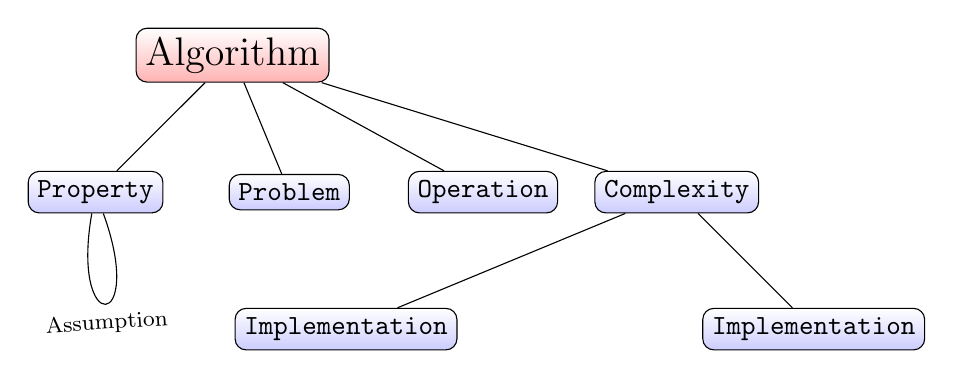
\begin{tikzpicture}
  [
    grow                    = right,
    node distance           = 7em,
    edge from parent/.style = {draw, -latex},
    every node/.style       = {font=\footnotesize},
    sloped
  ]
  \node [root] (0) {Algorithm};
  \node [env] (1) [below left of=0] {Property};
  \node [env] (2) [right of=1] {Problem};
  \node [env] (3) [right of=2] {Operation};
  \node [env] (4) [right of=3] {Complexity};
  \node [env] (5) [below left of=3] {Implementation};
  \node [env] (6) [below right of=4] {Implementation};

  \path [-]
    (0) edge (1)
    (0) edge (2)
    (0) edge (3)
    (0) edge (4)
    (4) edge (5)
    (4) edge (6)
    (1) edge [below, out=290, in=260, looseness=8, distance=1.6cm]
        node [swap] {Assumption} (1);
  
\end{tikzpicture}
\todo{Fix this caption, and figure, this was just proof of concept}
\caption{Explanation Tree for Dijkstra's 009}
\label{fig:djk-tree}
\end{figure}

\section{Discussion of Results}
In this section we summarize and interpret the results presented above. To
ensure transparency and openness, the reader may find all raw data, and all
encoded documents at \url{https://github.com/lambda-land/XOPTypology_Paper}.



\bibliography{XOPbib,eric}
\bibliographystyle{ACM-Reference-Format}

\end{document}
